\chapter{双星系统和恒星参数}
\section{双星分类}
\begin{itemize}
  \item 光学双星(optical double),只是观测看起来在一块,相互之间不受引力束缚
  \item 目视双星(visual binary),观测上能够直接分辨出两颗星
  \item 天测双星,伴星可能由于太暗不可见,但是可以从主星的运动情况分辨存在伴星
  \item 食双星,绕转轨道沿视线方向,会相互遮掩,能够观测到周期性的光度变化
  \item 光谱双星,具有独立、可分辨的光谱,可通过光谱分辨的双星,两颗星的光谱分别红移和蓝移
  \item 分光双星,周期短,可通过光谱的周期性红移分辨
\end{itemize}

以上分类并不相互独立,一个双星系统可以符合多种分类。

\section{目视双星测定质量}
第二章中提到多体运动可以使用质心参考系来研究,而在质心参考系中,位移矢量与质量存在关系(式\ref{eq:r}):
\begin{equation}
  {m_1\over m_2}={r_2\over r_1}={a_2\over a_1}
\end{equation}

上式$a$为椭圆轨道的长半轴,如果假定地球到该双星系统的距离$d$,且双星轨道平面垂直于视线,则可转化为质量$m$与角间距$\alpha$的关系:
\begin{equation}
  {m_1\over m_2}={a_2\over a_1}={\alpha_2 d\over \alpha_1 d}={\alpha_2\over \alpha_1}
\end{equation}

若双星轨道平面不垂直于视线,与垂直面存在倾角$i$,则上式变为
\begin{equation}
  {m_1\over m_2}={\alpha_2 \cos{i}\over \alpha_1\cos{i}}={\widetilde \alpha_2 \over \widetilde \alpha_1}
  \label{eq:binary1}
\end{equation}

同时考虑开普勒第三定律(式\ref{eq:kepler3})可得
\begin{equation}
  m_1+m_2={4\pi^2 \over G}{(\alpha d)^3 \over P^2}={4\pi^2\over G}\left({d\over \cos i}\right)^3{\widetilde \alpha^3\over P^3}
  \label{eq:binary2}
\end{equation}

其中$\widetilde \alpha=\widetilde \alpha_1+\widetilde \alpha_2$,结合式\ref{eq:binary1}和式\ref{eq:binary2}可得两颗恒星的质量。

\section{食双星和分光双星}
这种情况下一般只能得到一颗恒星的视向速度和周期,利用质心参考系的性质和开普勒第三定律,可以得到\textbf{质量函数}
\begin{equation}
  {m^3_2\over (m_1+m_2)^2}\sin^3 i={P\over 2\pi G}v^3_{1r}
\end{equation}

上式右边全是可观测量,若只能探测到一颗恒星的视向速度,则可以用上式得到$m_2$的下限,若可以探测到两颗恒星的视向速度,则结合下式可以计算两颗恒星的质量
\begin{equation}
  {m_1\over m_2}={v_{2r}/ \sin{i}\over v_{1r}\sin{i}}={v_{2r} \over v_{1r}}
\end{equation}

由于食双星和分光双星需要双星绕转平面与视线平行,才能够观测到足够的视向速度,所以通常可取$\langle\sin^3 i\rangle\simeq2/3$

\subsection{利用日食确定半径和温度比}
\begin{figure}[hbt]
  \centering
  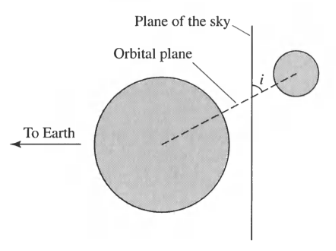
\includegraphics[width=6cm]{chapters/07/eclipse1}
  \caption{日食示意图,倾角$i$应接近90$^\circ$}
  \label{}
\end{figure}

\begin{figure}[hbt]
  \centering
  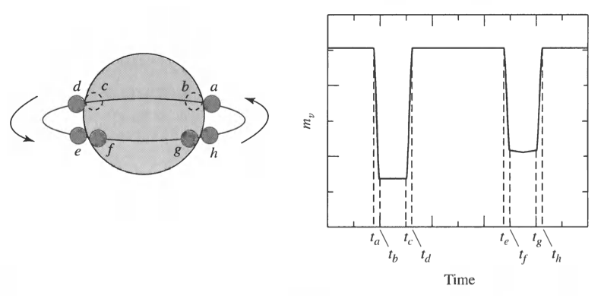
\includegraphics[width=12cm]{chapters/07/eclipse2}
  \caption{$i=90^\circ$(完全日食)的光变曲线,假设小恒星比大恒星更热}
  \label{}
\end{figure}

\begin{figure}[hbt]
  \centering
  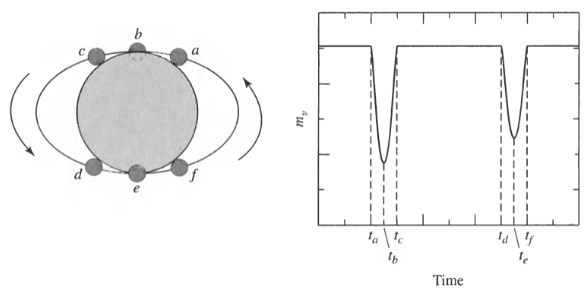
\includegraphics[width=12cm]{chapters/07/eclipse3}
  \caption{部分日食的光变曲线,假设小恒星比大恒星更热}
  \label{}
\end{figure}

由上图的光变曲线示意图可以得到两颗恒星的半径:
\begin{align}
  r_s&={v\over 2}(t_b-t_a)\\
  r_\ell &={v\over 2}(t_c-t_a)=r_s+{v\over 2}(t_c-t_b)
\end{align}

通过恒星半径以及斯特藩-玻尔兹曼公式(式\ref{eq:stefan}),可以得到温度$T$与亮度$B$的关系:
\begin{equation}
  {B_0-B_p\over B_0-B_s}=\left({T_e\over T_\ell}\right)^4
\end{equation}

其中$B_0$为两星分开的最大亮度,$B_p$为光变曲线的最小值,$B_s$为光变曲线的次极小值。
